\documentclass[a4paper, 12pt]{article}

%%% Работа с русским языком
\usepackage{cmap}					% поиск в PDF
\usepackage{mathtext} 				% русские буквы в формулах
\usepackage[T2A]{fontenc}			% кодировка
\usepackage[utf8]{inputenc}			% кодировка исходного текста
\usepackage[russian]{babel}	% локализация и переносы

%%% Дополнительная работа с математикой
\usepackage{amsmath,amsfonts,amssymb,amsthm,mathtools} % AMS
\usepackage{icomma} % "Умная" запятая: $0,2$ --- число, $0, 2$ --- перечисление

%% Номера формул
%\mathtoolsset{showonlyrefs=true} % Показывать номера только у тех формул, на которые есть \eqref{} в тексте.

%% Шрифты
\usepackage{euscript}	 % Шрифт Евклид
\usepackage{mathrsfs} % Красивый матшрифт

%% Поля
\usepackage[left=2cm,right=2cm,top=2cm,bottom=2cm,bindingoffset=0cm]{geometry}

%% Русские списки
\usepackage{enumitem}
\makeatletter
\AddEnumerateCounter{\asbuk}{\russian@alph}{щ}
\makeatother

%%% Работа с картинками
\usepackage{graphicx}  % Для вставки рисунков
\graphicspath{{images/}{images2/}}  % папки с картинками
\setlength\fboxsep{3pt} % Отступ рамки \fbox{} от рисунка
\setlength\fboxrule{1pt} % Толщина линий рамки \fbox{}
\usepackage{wrapfig} % Обтекание рисунков и таблиц текстом

%%% Работа с таблицами
\usepackage{array,tabularx,tabulary,booktabs} % Дополнительная работа с таблицами
\usepackage{longtable}  % Длинные таблицы
\usepackage{multirow} % Слияние строк в таблице
\usepackage[table,xcdraw]{xcolor} % Цветные таблицы

%% Красная строка
\setlength{\parindent}{2em}

%% Интервалы
\linespread{1}
\usepackage{multirow}

%% TikZ
\usepackage{tikz}
\usetikzlibrary{graphs,graphs.standard}

%% Верхний колонтитул
\usepackage{fancyhdr}
\pagestyle{fancy}

%% Перенос знаков в формулах (по Львовскому)
\newcommand*{\hm}[1]{#1\nobreak\discretionary{}
	{\hbox{$\mathsurround=0pt #1$}}{}}

%% Мои дополнения
\usepackage{float} %Добавляет возможность работы с командой [H] которая улучшает расположение на странице
\usepackage{gensymb} %Красивые градусы
\usepackage{graphicx}               % Импорт изображений
\usepackage{caption} % Пакет для подписей к рисункам, в частности, для работы caption*


\begin{document}

\newcommand{\HRule}{\rule{\linewidth}{0.7mm}} % Defines a new command for the horizontal lines, change thickness here
	
	\begin{center}
		\large\textbf{Московский Физико-Технический Институт}\\
		\large\textbf{(государственный университет)}
	
		\vfill
		
		\Large Лабораторная работа по радиотехническим сигналам и цепям № 20\\[0.5cm] % Minor heading such as course title
		
		%----------------------------------------------------------------------------------------
		%	TITLE SECTION
		%----------------------------------------------------------------------------------------
		
		\HRule
		\\[0.4cm]
		{ \huge \bfseries Связанные колебательные контуры}
		\\[0.4cm] % Title of your document
		\HRule
		\\[0.5cm]
		
		\ \\
	\textbf{\large Автор:} \\	
	\large Баранников Андрей Б01-001\\
	\textbf{\large Преподаватель:} \\
	\large Григорьев Иван Александрович\\
		\vfill
		\hspace*{-0.8 cm}
\includegraphics[width=100 pt]{frkt_logo}\\
		\large Долгопрудный, 2021
	\end{center}

\newpage
\setcounter{page}{2}
\fancyfoot[c]{\thepage}
\fancyhead[L] {Работа № 20}
\fancyhead[R]{}
\newpage 
\section*{Задание 1.1}

\begin{enumerate}
	\item Исследую модель резистора как источника шумового напряжения. Для этого установлю $\{E_s/ne\}$. Убедимся, что графики шумовых напряжений на выходе и входе равны. С помощью варьирования резистора убедимся, что шум растёт как $\sqrt{R}$.
	
	\item Подключим график корня из интеграла от спектральной плотности и измерим эффективное напряжение шума $\sigma$ на выводах резисторов: 
	
	\begin{table}[!h]
		\centering
		\begin{tabular}{|cc|cc|}
			\hline
			\multicolumn{2}{|c|}{R   {[}1k, 16k|Log2{]}} & \multicolumn{2}{c|}{R {[}1k, 1000k|Log10{]}} \\ \hline
			\multicolumn{1}{|c|}{R, кОм}   & $\sigma$, мкВ  & \multicolumn{1}{c|}{R, кОм}   & $\sigma$, мкВ   \\ \hline
			\multicolumn{1}{|c|}{1}        & 4           & \multicolumn{1}{c|}{1}        & 4            \\ \hline
			\multicolumn{1}{|c|}{2}        & 5,7         & \multicolumn{1}{c|}{10}       & 13           \\ \hline
			\multicolumn{1}{|c|}{4}        & 8           & \multicolumn{1}{c|}{100}      & 40           \\ \hline
			\multicolumn{1}{|c|}{8}        & 11,5        & \multicolumn{1}{c|}{1000}     & 130          \\ \hline
			\multicolumn{1}{|c|}{16}       & 16,2        &                               &              \\ \hline
		\end{tabular}
		\caption{Зависимость эффективного напряжения $\sigma$ от $R$}
		\label{tab:table_1}
	\end{table}

	\item Перейдём к модели источника тока. Варьируя $R_1$ проверим, что шумовое напряжение растёт как $\sqrt{R}$, а ток падает как $1/\sqrt{R}$:
	
	\begin{table}[!h]
		\centering
		\begin{tabular}{|c|c|c|c|c|}
			\hline
			R, кОм & 1    & 2    & 4    & 8     \\ \hline
			e, нВ  & 4,00 & 5,80 & 8,00 & 10,00 \\ \hline
			I, пА  & 4,00 & 2,90 & 2,00 & 1,25  \\ \hline
		\end{tabular}
		\caption{Зависимость шумового напряжения $e$ и тока $i$ от $R$}
		\label{tab:table_2}
	\end{table}

	Как видим, предположение зависимости подтверждается данными.\\

\end{enumerate}

\section*{Задание 1.2}

\begin{enumerate}
	\item Проверим закон сложения шумовых токов для последовательного соединения варьируя $R_1$ и $R_2$:
		\[
			e_1 = \sqrt{4ktR_2} = 5,8 \ нВ \quad \quad e_2 = \sqrt{4ktR_1} = 4 \ нВ \quad \quad e_{об \ эксп} = 7 \ нВ
		\]
		\[
			e_{об \ теор} = \sqrt{4kt(R_1 + R_2)} = \sqrt{5,8^2 + 4^2} \approx 7,05 \ нВ \quad \Rightarrow \quad \boxed{e_{об \ эксп} = e_{об \ теор}}
		\]
	
	\item Проверим закон сложения шумовых токов для параллельного соединения:
	\[
		e_3 = \sqrt{4kTR_3} \approx 5,8 \ нВ \quad \quad e_4 = \sqrt{4kTR_4} \approx 4,1 \ нВ \quad \quad e_{об \ эксп} = 3,35 \ нВ
	\]
	\[
		e_{об \ теор} = \sqrt{4kT (R_3 || R_4)} = \sqrt{4kT \frac{R_3 R_4}{R_3 + R_4}} = \sqrt{\frac{e_3^2 \cdot e_4^2}{e_3^2 + e_4^2}} = \sqrt{\frac{5,8^2 \cdot 4^2}{5,8^2 + 4^2}} = 3,30
	\]
	\[
		\boxed{e_{об \ эксп} = e_{об \ теор}}
	\]
	
\end{enumerate}

\newpage
\section*{Задание 1.3}

\begin{enumerate}
	\item Изучу зависимость приведённого ко входу напряжения от сопротивления $ R $. Построю графики зависимости от $ R $ коэффициента шума $ K_n $ делителя и шумовой температуры $ T_n $.
	
	\begin{table}[!h]
		\centering
		\begin{tabular}{|c|c|c|}
			\hline
			R, кОм & K\_n, дБ & T\_n, K \\ \hline
			2      & 7,04     & 1219    \\ \hline
			4      & 4,80      & 606     \\ \hline
			8      & 3,02     & 302     \\ \hline
			16     & 1,89     & 163     \\ \hline
			32     & 0,96     & 74      \\ \hline
		\end{tabular}
		\caption{Данные о сопротивлении $ R $,  коэффициенте шума $ K_n $, и шумовой температуре $ T_n $}
		\label{tab:table_3}
	\end{table}
	\begin{figure}[h!]
		\centering 
		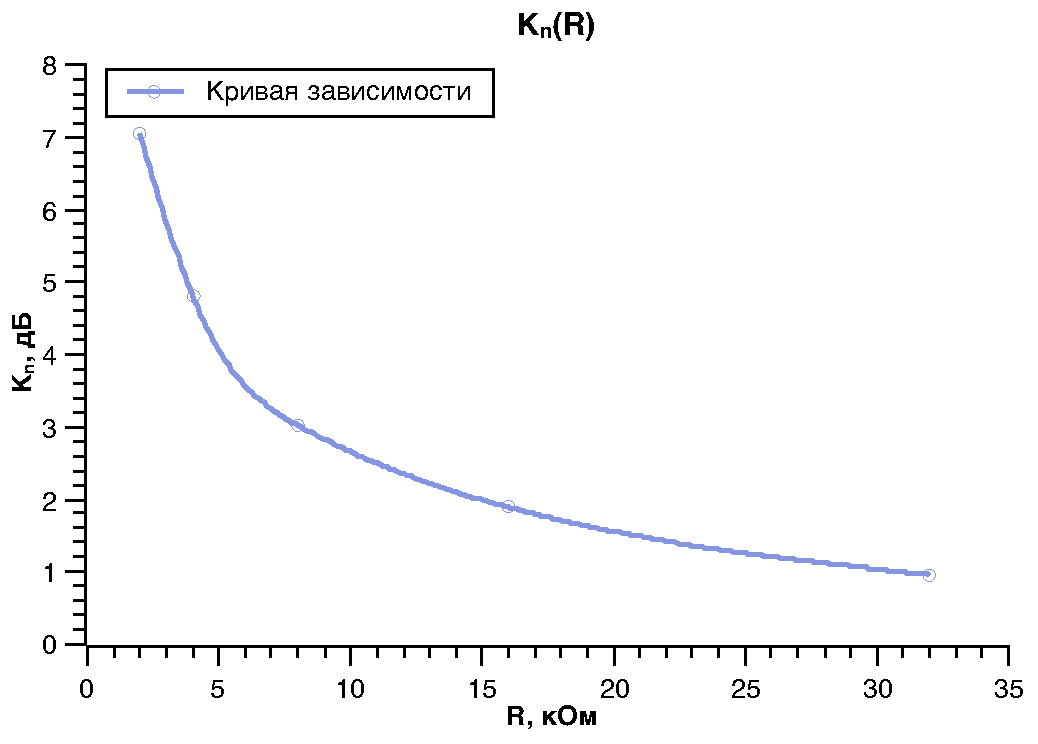
\includegraphics[width = 0.5\linewidth]{plot_1}
		\caption{Зависимость коэффициента шума $ K_n $ от сопротивления $ R $}
		\label{fig:plot_1}
	\end{figure}

	\begin{figure}[h!]
		\centering 
		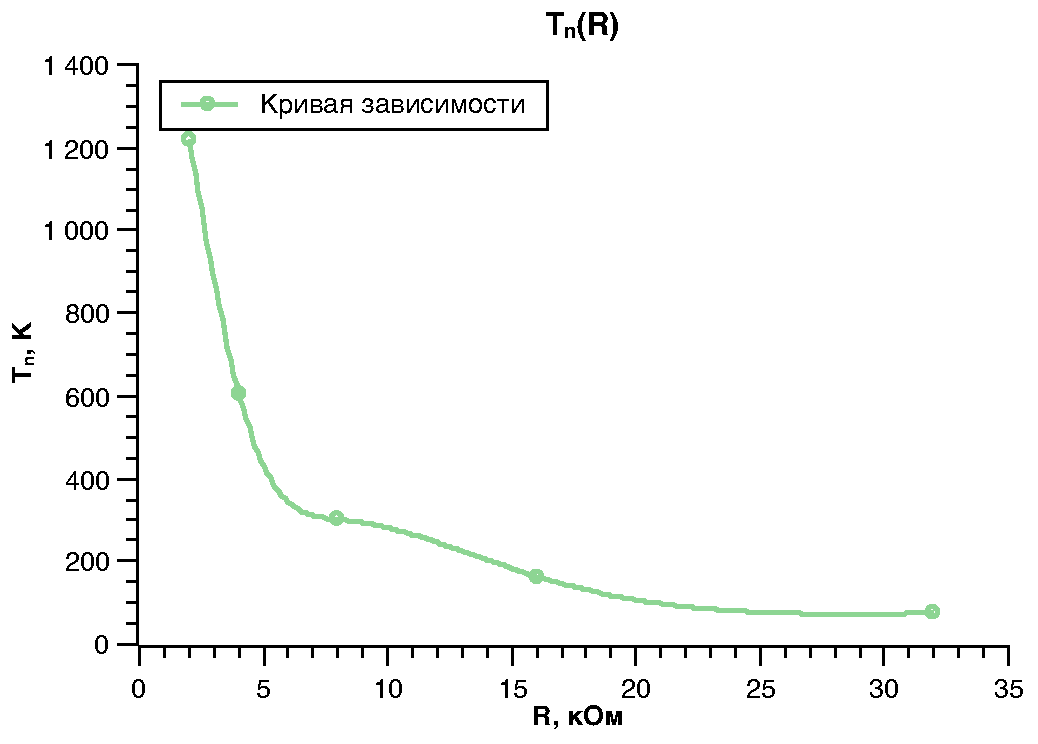
\includegraphics[width = 0.5\linewidth]{plot_2}
		\caption{Зависимость шумовой температуры $ T_n $ от сопротивления $ R $}
		\label{fig:plot_2}
	\end{figure}


	
	\item При исключении из схемы резистора $ R $ и установке вместо него нешумящего резистора H, отношение сигнал/шум не ухудшается, так как по анализу схемы видно, что $ e =  e_n $	
	
\end{enumerate}

\newpage
\section*{Задание 2}
\begin{enumerate}
	\item Изучим зависимость дробового тока от $ I_0 $ в области микротоков и умеренных токов. Проверим выполнение закона $ \sqrt{I_0} $.
	
	\begin{table}[!h]
		\centering
		\begin{tabular}{|cc|cc|}
			\hline
			\multicolumn{2}{|c|}{$ I_0 $ {[}1u,   1m|Log10{]}} & \multicolumn{2}{c|}{$ I_0 $ {[}1m, 32m|Log2{]}} \\ \hline
			\multicolumn{1}{|c|}{$ i $, пA}     & $ I_0 $, мкА    & \multicolumn{1}{c|}{$ i $, пA}    & $ I_0 $, мА    \\ \hline
			\multicolumn{1}{|c|}{0,606}     & 1            & \multicolumn{1}{c|}{17,6}     & 1           \\ \hline
			\multicolumn{1}{|c|}{1,817}     & 10           & \multicolumn{1}{c|}{25,2}     & 2           \\ \hline
			\multicolumn{1}{|c|}{5,700}     & 100          & \multicolumn{1}{c|}{35,0}     & 4           \\ \hline
			\multicolumn{1}{|c|}{17,811}    & 1000         & \multicolumn{1}{c|}{49,0}     & 8           \\ \hline
			&              & \multicolumn{1}{c|}{67,5}     & 16          \\ \cline{3-4} 
			&              & \multicolumn{1}{c|}{90,5}     & 32          \\ \hline
		\end{tabular}
		\caption{Измерения дробового тока в зависимости от $ I_0 $}
		\label{tab:table_4}
	\end{table}
	Напряжение пробоя диода: $ \boxed{U_{пр} = 100,6 \ В} $

	\item Измерим значения дифференциального сопротивления диода $ r_d $  при варьировании $ I_1 $: 
	
	\begin{table}[!h]
		\centering
		\begin{tabular}{|c|c|c|}
			\hline
			$ I_1 $, мкА & $ K $    & $ r_d $, кОм \\ \hline
			1000      & 0,008 & 0,08        \\ \hline
			100       & 0,050 & 0,53        \\ \hline
			10        & 0,341 & 5,17        \\ \hline
			1         & 0,838 & 51,73        \\ \hline
		\end{tabular}
	\caption{Измерение дифференциального сопротивления $ r_d $ при варьировании $ I_1 $ }
	\label{tab:table_5}
	\end{table}

	\item Измерим уровени шумового напряжения $ e(f) $ для варьирования $ I_1 $. По результатам измерений проверим выполнение равенства $ e(f) = i(f) r_d $
	
	\begin{table}[!h]
		\centering
		\begin{tabular}{|c|c|c|}
			\hline
			$ r_d $, кОм & $ e(f)_{эксп} $, нВ & $ e(f)_{теор} $, нВ \\ \hline
			0,08      & 1,0            & 1,4            \\ \hline
			0,53      & 3,0            & 3,0            \\ \hline
			5,17      & 9,3            & 9,4            \\ \hline
			51,73     & 30,0           & 31,3           \\ \hline
		\end{tabular}
		\caption{Проверяем соотносимость теоритического и экспериментального $ e(f) $}
		\label{tab:table_6}
	\end{table}

	\item При $ I_1 < 100 \ нА $ не получается сохранить полосу шума не хуже 100 кГц. Максимальное напряжение в таком режиме $ u = 332 \ мкВ $. \\
			Искомые значения вне диапозона: 
			\[
				\boxed{I = 270 \ нА} \quad \quad \boxed{u = 60 \ нА} \quad \quad \boxed{\sigma = 19,2}
			\] 
\end{enumerate}

\newpage

\section*{Задание 3}

\begin{enumerate}
	\item Интегрирующая цепь
	\[
		f_h = 10 \ кГц \quad \quad n_1 = 13 \ нА \quad \quad \sigma = 1,6 \ мкВ
	\]
	\[
		\sigma_{теор} = 13 \ нА \ \sqrt{\frac{\pi \cdot 10 \ кГц}{2}} \approx 1,63 \ мкВ
	\]
	\begin{table}[!h]
		\begin{minipage}[h]{0.45\linewidth}
				\centering
				\begin{tabular}{|cc|}
					\hline
					\multicolumn{2}{|c|}{$ R_1 $ {[}2k, 16k|4k{]}} \\ \hline
					\multicolumn{1}{|c|}{$ R_1 $, кОм}    & $ n_1 $, нВ    \\ \hline
					\multicolumn{1}{|c|}{2}          & 5,9     \\ \hline
					\multicolumn{1}{|c|}{6}          & 9,8      \\ \hline
					\multicolumn{1}{|c|}{10}         & 12,8     \\ \hline
					\multicolumn{1}{|c|}{14}         & 15,3     \\ \hline
					\multicolumn{1}{|c|}{16}         & 16,3     \\ \hline
				\end{tabular}
				\caption{Зависимость шумового напряжения $ n_1 $ от $ R_1 $}
				\label{tab:table_7}
		\end{minipage}
		\hfill
		\begin{minipage}[h]{0.45\linewidth}
			\centering
			\begin{tabular}{|ccc|}
				\hline
				\multicolumn{3}{|c|}{$ C_1 $   {[}0.8n, 2.4n|0,4n{]}}                          \\ \hline
				\multicolumn{1}{|c|}{$ C_1 $, нФ} & \multicolumn{1}{c|}{$ n_1 $, нВ} & $ \sigma $, мкВ \\ \hline
				\multicolumn{1}{|c|}{0,8}      & \multicolumn{1}{c|}{2,3}      & 0,28       \\ \hline
				\multicolumn{1}{|c|}{1,2}      & \multicolumn{1}{c|}{1,9}      & 0,23       \\ \hline
				\multicolumn{1}{|c|}{1,6}      & \multicolumn{1}{c|}{1,6}      & 0,20       \\ \hline
				\multicolumn{1}{|c|}{2,0}      & \multicolumn{1}{c|}{1,5}      & 0,18       \\ \hline
				\multicolumn{1}{|c|}{2,4}      & \multicolumn{1}{c|}{1,3}      & 0,16       \\ \hline
			\end{tabular}
			\caption{Зависимость уровня шума $ \sigma $  от ёмкости $ C $}
			\label{tab:table_8}
		\end{minipage}
	\end{table}

	Уровень шума не зависит от $ R_1 $, потому что выражается формулой $ P = \frac{k T}{C} $

	\item Полосовой LC-фильтр 
	\[
		f_0 = 100 \ кГц \quad \quad \Delta f = 18 \ кГц \quad \quad Q = \frac{f_0}{\Delta f} = 5,5
	\]
	\[
		n_2 = 10,2 \ нВ \quad \quad \sigma_{эксп} = 1,8 \ мкВ \quad \quad \sigma_{теор} = 10,2 \ нВ \cdot \sqrt{\frac{\pi \cdot 100 \ кГц}{2 \cdot 5,5}} \approx 1,73 \ мкВ
	\]
	
	\begin{table}[!h]
		\begin{minipage}[h]{0.45\linewidth}
			\centering
			\begin{tabular}{|cc|}
				\hline
				\multicolumn{2}{|c|}{$ R_2 $ {[}2.3k, 10.3k|4k{]}}   \\ \hline
				\multicolumn{1}{|c|}{$ n_2(f_0) $, нВ} & $ R_2 $, кОм \\ \hline
				\multicolumn{1}{|c|}{6,3}             & 2,3       \\ \hline
				\multicolumn{1}{|c|}{10,0}            & 6,3       \\ \hline
				\multicolumn{1}{|c|}{12,9}            & 10,3      \\ \hline
			\end{tabular}
			\caption{Зависимость шумового напряжения $ n_2(f_0) $ от $ R_2 $}
			\label{tab:tabel_9}
		\end{minipage}
		\hfill
		\begin{minipage}[h]{0.45\linewidth}
			\centering
			\begin{tabular}{|cc|}
				\hline
				\multicolumn{2}{|c|}{$ С_2 $ {[}0.75n, 1.75n|0.5n{]}} \\ \hline
				\multicolumn{1}{|c|}{$ C_2 $, нФ}    & $ \sigma $,  мкВ   \\ \hline
				\multicolumn{1}{|c|}{0,75}        & 2,34          \\ \hline
				\multicolumn{1}{|c|}{1,25}        & 1,8           \\ \hline
				\multicolumn{1}{|c|}{1,75}        & 1,53          \\ \hline
			\end{tabular}
			\caption{Зависимость уровня шума $ \sigma $ от $ C_2 $}
			\label{tab:tabel_10}
		\end{minipage}
	\end{table}

	\item LC-фильтр нижних частот
	\[
		f_0 = 100 \ кГц \quad \quad n_3(f_0) = 10,3 \ нВ \quad \quad n_3(f_0/10) = 2 \ нВ \quad \quad \sigma_{вых} = 1,8 \ мкВ
	\]
	\[
	F_{n \ эксп} = \left(\frac{\sigma}{n}\right)^2 \approx 30540 \quad \quad F_{n \ теор} = \frac{\pi}{2} \frac{f_0}{Q} \approx 31415
	\]
	 
	 \newpage
	\begin{table}[!h]
		\centering
		\begin{tabular}{|cccc|}
			\hline
			\multicolumn{4}{|c|}{$ R_3 $ {[}100, 400|150{]}}                                                                                         \\ \hline
			\multicolumn{1}{|c|}{$ R_3 $, Ом} & \multicolumn{1}{c|}{$ n_3(f_0) $, нВ} & \multicolumn{1}{c|}{$ n_3 (f_0/10) $, нВ} & $ \sigma $, мкВ           \\ \hline
			\multicolumn{1}{|c|}{100}      & \multicolumn{1}{c|}{16,2}           & \multicolumn{1}{c|}{1,3}               & \multirow{3}{*}{1,8} \\ \cline{1-3}
			\multicolumn{1}{|c|}{250}      & \multicolumn{1}{c|}{10,5}           & \multicolumn{1}{c|}{2,0}               &                      \\ \cline{1-3}
			\multicolumn{1}{|c|}{400}      & \multicolumn{1}{c|}{8,3}            & \multicolumn{1}{c|}{2,6}               &                      \\ \hline
		\end{tabular}
		\caption{Зависимость величин при варьировании $ R $}
		\label{tab:tabel_11}
		
		\begin{tabular}{|cccc|}
			\hline
			\multicolumn{4}{|c|}{$ C_3 $ {[}0.75n, 1.75n| 0,5n{]}}                                                                          \\ \hline
			\multicolumn{1}{|c|}{$ C_3 $, нФ} & \multicolumn{1}{c|}{$ n_3 (f_0) $, нВ} & \multicolumn{1}{c|}{$ n_3(f_0/10) $, нВ}  & $ \sigma $, мкВ \\ \hline
			\multicolumn{1}{|c|}{0,75}     & \multicolumn{1}{c|}{13,3}           & \multicolumn{1}{c|}{\multirow{3}{*}{2}} & 2,3        \\ \cline{1-2} \cline{4-4} 
			\multicolumn{1}{|c|}{1,25}     & \multicolumn{1}{c|}{10,3}           & \multicolumn{1}{c|}{}                   & 1,8        \\ \cline{1-2} \cline{4-4} 
			\multicolumn{1}{|c|}{1,75}     & \multicolumn{1}{c|}{8,8}            & \multicolumn{1}{c|}{}                   & 1,5        \\ \hline
		\end{tabular}
		\caption{Зависимость величин при варьировании $ C $}
		\label{tab:tabel_12}

		\begin{tabular}{|cccc|}
			\hline
			\multicolumn{4}{|c|}{$ L_3 ${[}1m, 3m|1m{]}}                                                                                             \\ \hline
			\multicolumn{1}{|c|}{$ L_3 $, мГн} & \multicolumn{1}{c|}{$ n_3 (f_0) $, нВ} & \multicolumn{1}{c|}{$ n_3(f_0/10) $, нВ}  & $ \sigma $, мкВ           \\ \hline
			\multicolumn{1}{|c|}{1}         & \multicolumn{1}{c|}{7,4}            & \multicolumn{1}{c|}{\multirow{3}{*}{2}} & \multirow{3}{*}{1,8} \\ \cline{1-2}
			\multicolumn{1}{|c|}{2}         & \multicolumn{1}{c|}{10,4}           & \multicolumn{1}{c|}{}                   &                      \\ \cline{1-2}
			\multicolumn{1}{|c|}{3}         & \multicolumn{1}{c|}{12,6}           & \multicolumn{1}{c|}{}                   &                      \\ \hline
		\end{tabular}
		\caption{Зависимость величин при варьировании $ L $}
		\label{tab:tabel_13}
		\end{table}
	
	\item LC-фильтр верхних частот
	\[
		f_0 = 100 \ кГц \quad \quad n_4(f_0) = 10,3 \ нВ \quad \quad n_4(10f_0) = 2 \ нВ \quad \quad \sigma = 2,7 \ мкВ
	\]
	
	\begin{table}[!h]
		\centering
		\begin{tabular}{|cccc|}
			\hline
			\multicolumn{4}{|c|}{$ R_4 $ [100, 400|150]}                                                                              \\ \hline
			\multicolumn{1}{|c|}{$ R_4 $, Ом} & \multicolumn{1}{c|}{$ n_3(f_0) $, нВ} & \multicolumn{1}{c|}{$ n_3(10f_0) $, нВ} & $ \sigma $, мкВ \\ \hline
			\multicolumn{1}{|c|}{100}     & \multicolumn{1}{c|}{16,3}         & \multicolumn{1}{c|}{1,3}            & 2,2        \\ \hline
			\multicolumn{1}{|c|}{250}     & \multicolumn{1}{c|}{10,4}         & \multicolumn{1}{c|}{2,0}              & 2,7        \\ \hline
			\multicolumn{1}{|c|}{400}     & \multicolumn{1}{c|}{8,3}          & \multicolumn{1}{c|}{2,6}            & 3,0          \\ \hline
		\end{tabular}
		\caption{Зависимость величин при варьировании $ R $}
		\label{tab:tabel_14}
		
		\begin{tabular}{|cccc|}
			\hline
			\multicolumn{4}{|c|}{$ С_4 $[0.75n, 1.75n|0.5n]}                                                                             \\ \hline
			\multicolumn{1}{|c|}{$ C_4 $, нФ} & \multicolumn{1}{c|}{$ n_3(f_0) $, нВ} & \multicolumn{1}{c|}{$ n_3(10f_0) $, нВ}     & $ \sigma $, мкВ \\ \hline
			\multicolumn{1}{|c|}{0,75}    & \multicolumn{1}{c|}{13,3}         & \multicolumn{1}{c|}{\multirow{3}{*}{2}} & 3          \\ \cline{1-2} \cline{4-4} 
			\multicolumn{1}{|c|}{1,25}    & \multicolumn{1}{c|}{10,3}         & \multicolumn{1}{c|}{}                   & 2,7        \\ \cline{1-2} \cline{4-4} 
			\multicolumn{1}{|c|}{1,75}    & \multicolumn{1}{c|}{8,8}          & \multicolumn{1}{c|}{}                   & 2,5        \\ \hline
		\end{tabular}
		\caption{Зависимость величин при варьировании $ C $}
		\label{tab:tabel_15}
		
		\begin{tabular}{|cccc|}
			\hline
			\multicolumn{4}{|c|}{$ L_4 $ [1m, 3m|1m]}                                                                                                \\ \hline
			\multicolumn{1}{|c|}{$ L_4 $, мГн} & \multicolumn{1}{c|}{$ n_3(f_0) $, нВ} & \multicolumn{1}{c|}{$ n_3(10f_0) $, нВ}     & $ \sigma $, мкВ           \\ \hline
			\multicolumn{1}{|c|}{1}        & \multicolumn{1}{c|}{7,3}          & \multicolumn{1}{c|}{\multirow{3}{*}{2}} & \multirow{3}{*}{2,7} \\ \cline{1-2}
			\multicolumn{1}{|c|}{2}        & \multicolumn{1}{c|}{10,3}         & \multicolumn{1}{c|}{}                   &                      \\ \cline{1-2}
			\multicolumn{1}{|c|}{3}        & \multicolumn{1}{c|}{12,6}         & \multicolumn{1}{c|}{}                   &                      \\ \hline
		\end{tabular}
		\caption{Зависимость величин при варьировании $ L $}
		\label{tab:tabel_16}
		
	\end{table}
	
\end{enumerate}

\newpage

\section*{Задание 4.3}
\[
	f_0 = 100 \ кГц \quad \quad \Delta f = 34 \ кГц \quad \quad K_{рез} = 0,5 \quad \quad K_{0} = 0,029
\]

\begin{figure}[h!]
	\centering
	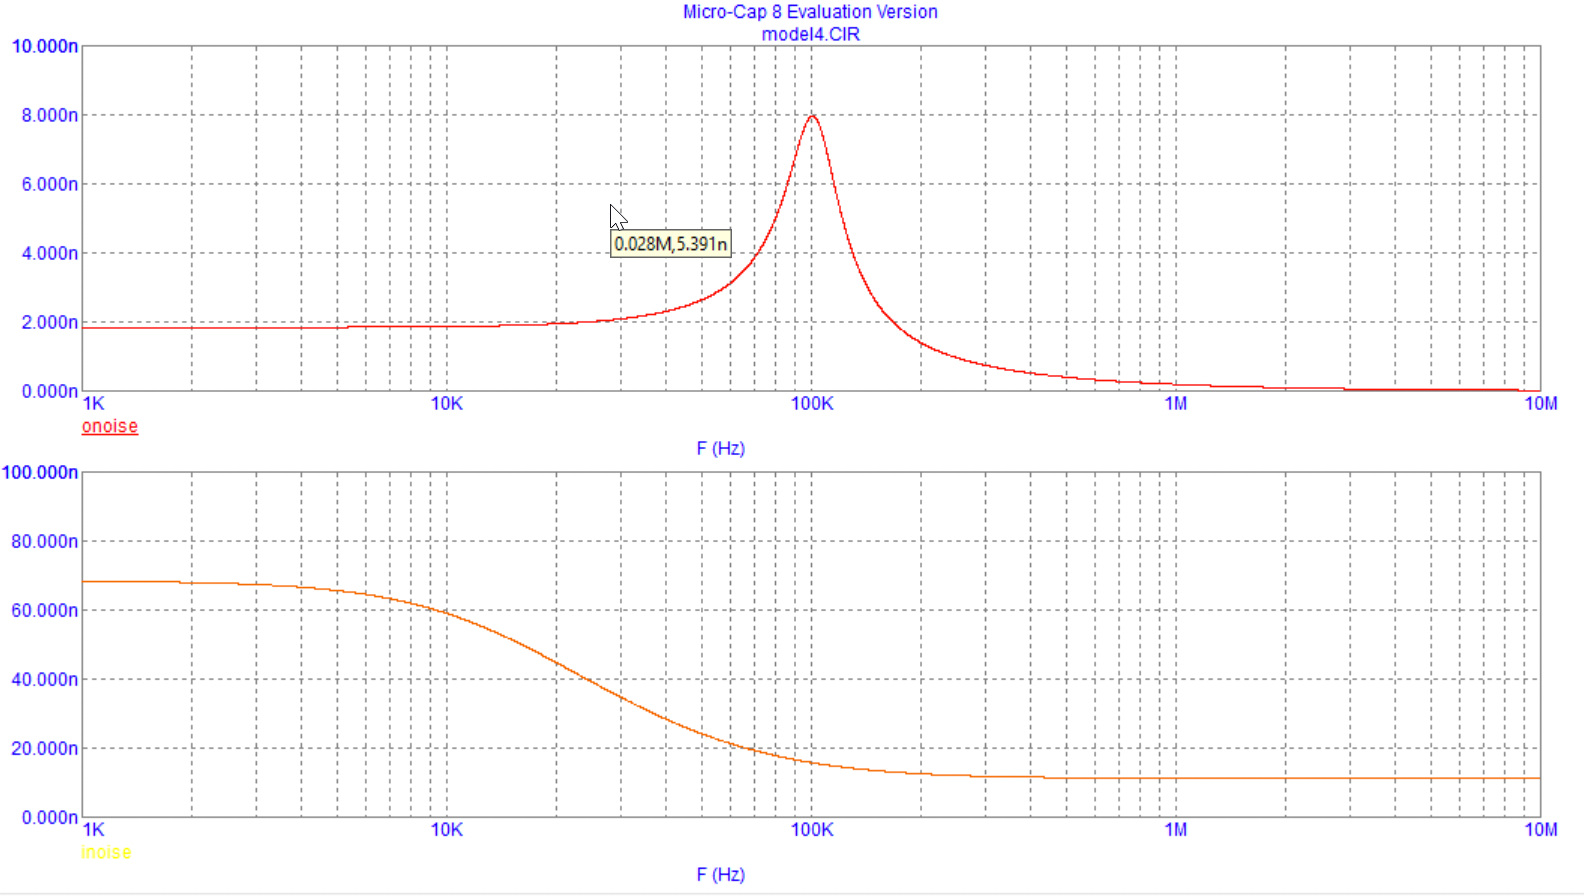
\includegraphics[width = \textwidth]{image_1}
	\caption{График шумового напряжения на выходе $ n_3 $}
	\label{fig:image_1}
\end{figure}

На низких частотах шум на выходе создаётся параллельным соединением $ r||R $ и отличен от нуля. Малый коэффициент передачи даёт высокий уроыень шума. Всё это возможно, так как на низких частотах индуктивный импеданс мал, а ёмкостный велик. Если же увеличить частоту, индуктивный импеданс "отключает" резистор $ r $, это приводит к вырождению цепь в интегрирующую с нулевым коэффициентом шума. В резонансе же наблюдается выброс. \\ 
\begin{itemize}
	\item Уровни шумового напряжения на разных частотах: 
		\[
		n(f_0) = 8,0 \ нВ \quad \quad n(f_0/100) = 1,9 \ нВ
		\]
	\item Оценим вклады шумов резисторов:
		\[
			n_1(f) - вклад \ R_{s3} \quad \quad n_2(f) - вклад \ R_{3} \ - \ в \ шумовое \ напряжение
		\]
		\[
			\sigma_1 - вклад \ R_{s3} \quad \quad \sigma_2 - вклад \ R_{3} \ - \ в \ уровень \ шума \ на \ выходе
		\]
		\[
			n_1(f_0) = 5,4 \ нВ \quad \quad n_1(f_0/100) = 0,3 \ нВ \quad \quad n_2(f_0) = 0,340 \ нВ \quad \quad n_2(f_0/100) = 1,0 \ нВ
		\]
		\[
			\sigma_1 = 1,3 \ мкВ \quad \quad \sigma_2 = 230 \ нВ
		\]
	\item Оценим значение коэффициента шума на различных частотах:
	\[
		K_n = 20 \lg \frac{e_n(f)}{\sqrt{4kTR}} \quad \Rightarrow \quad K_n(f_0/100) \approx 16 \quad \quad K_n(f_0) \approx 3 \quad \quad K_n(10f_0) \approx 0
	\]
\end{itemize}

\newpage 
\section*{Вывод коэффициентов передачи}
\begin{figure}[h!]
	\centering
	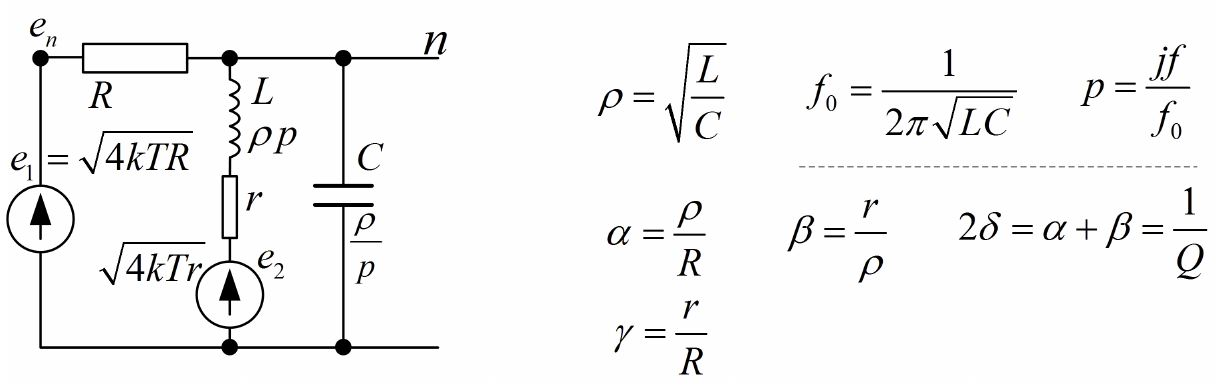
\includegraphics[width = \textwidth]{image_2}
	\caption{LC Фильтр нижних частот}
	\label{fig:image_2}
\end{figure}
\[
	K_1 = \frac{n}{e_1}
\]
\[
	Z_{об} = R + Z_{||} \quad \quad Z_{||} = \frac{\rho(\rho p + r)}{p(\rho p + r) + \rho} \quad \Rightarrow \quad I = \frac{e_1}{Z_{об}}
\]
\[
	e_1 - IR = n \quad \Rightarrow \quad e_1 - e_1 \frac{R}{Z_{об}} = n \quad \Rightarrow \quad \frac{n}{e_1} = \frac{Z_{||}}{Z_{об}}
\]
\[
Z_{об} = \frac{ (\rho p + r)( Rp + \rho ) + R \rho}{ p(\rho p + r) + \rho }
\]
\[
K_1 = \frac{n}{e_1} = \frac{\rho^2 p + \rho r}{(\rho p + r)(R p + \rho) + R \rho} = \frac{\frac{\rho p}{R} + \frac{r}{R}}{p^2 + \rho\frac{p}{R} + r \frac{p}{\rho} + \frac{r}{R} + 1} 
\]
\[
\boxed{K_1 = \frac{\gamma + \alpha p}{p^2 + 2 \delta p + 1 + \gamma}}
\]
\[
K_2 = \frac{n}{e_2}
\]
\[
Z_{об} = r + \rho p + Z_{||} \quad \quad Z_{||} = \frac{R \rho}{Rp + \rho} \quad \quad I = \frac{e_2}{Z_{об}} = \frac{e_2}{r + \rho p + Z_{||}}
\]
\[
I \cdot Z_{||} = n \quad \Rightarrow \quad e_2\frac{Z_{||}}{r + \rho p + Z_{||}} = n \quad \Rightarrow \quad \frac{n}{e_2} = \frac{Z_{||}}{r + \rho p + Z_{||}}
\]
\[
K_2 = \frac{n}{e_2} = \frac{R \rho}{Rp + \rho} \cdot \frac{1}{r + \rho p + \frac{R \rho}{Rp + \rho}} = \frac{R\rho}{Rrp + r \rho + R p^2 \rho + \rho^2 p + R \rho} = \frac{1}{\frac{rp}{\rho} + \frac{r}{R} + p^2 \frac{\rho p}{R} + 1}
\]

\[
\boxed{K_2 = \frac{1}{p^2 + 2\delta p + 1 \gamma}}
\]
\end{document}